
The electrical model consists of low-voltage (LV) and high-voltage (HV) circuits, depicted in
Fig.~\ref{electrical_model}. The LV current (supplied at 11~V) is used to power the hybrid controller chips (HCCs),
ATLAS Binary Chips (ABCs) and Autonomous Monitoring and Control chip (AMAC) located on PCBs that are
glued directly onto the surface of the sensor.
These chips require between 1.5 and 3.3~V, which are provided by the temperature-dependent
FEAST DC-DC converter (labeled bPOL12V in Fig.~\ref{electrical_model}) and an LDO (low-dropout) regulator (labeled bPOL12).
The number of chips and converters on each module vary according to the design of
each different module type (barrel short-strip and long-strip modules, and six different endcap
module designs).
A barrel or endcap module contains 10--28 ABC chips, 1--4 HCCs, and
1--2 of each of the other components (linPOL12V/bPOL12V/AMAC).

\begin{figure}[ht!]
\centering
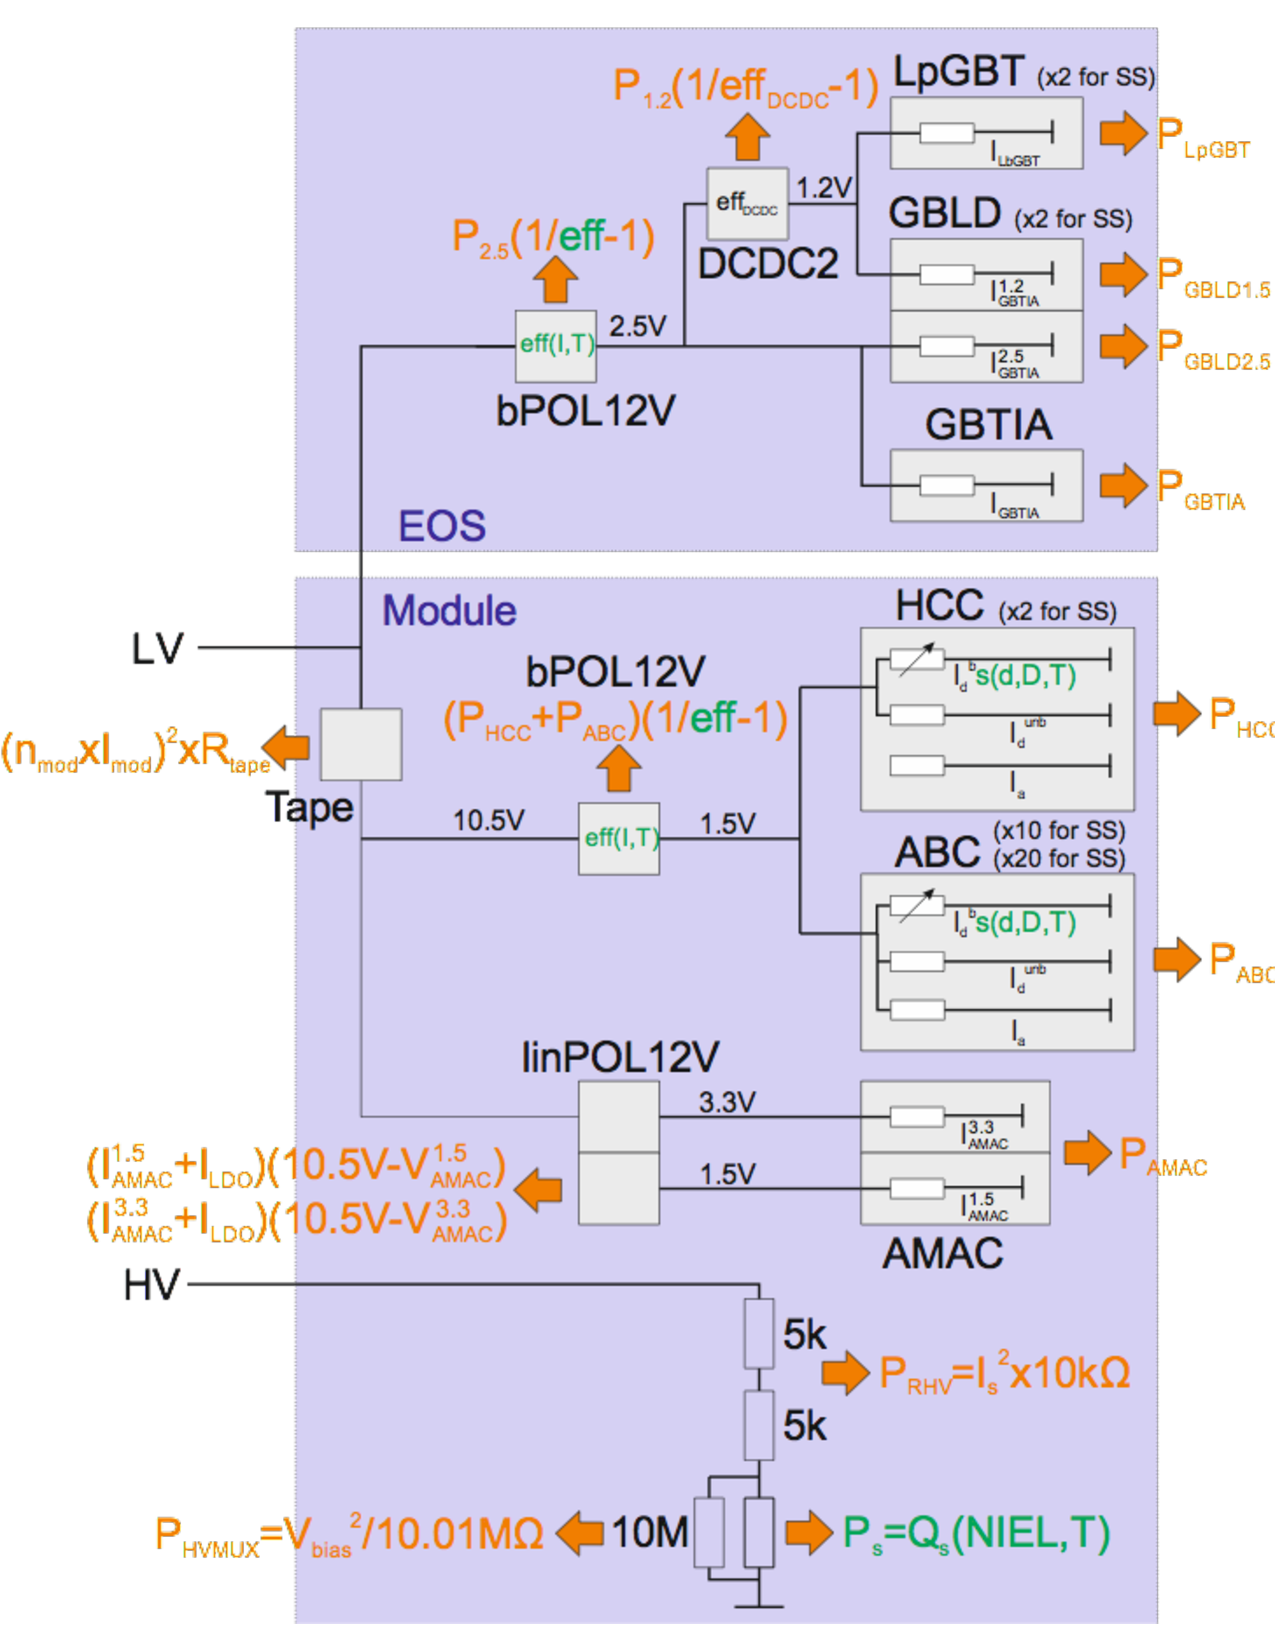
\includegraphics[width=0.8\linewidth]{figures/electrical_model.pdf}
\caption{
The electrical model of the ITk Strip barrel and endcap modules. Green arrows represent temperature-dependent heat sources, while orange arrows are temperature-independent. Grey squares are chips.
% Chip counts per module are linPOL12V/bPOL12/AMAC: 1 each (2 each for EC R3); HCC: 1 for barrel LS, 2 for barrel SS and EC R0-R2 and R4-R5, 4 for EC R3; ABC: barrel: 10, 20 (LS, SS), EC: 17, 21, 21, 28, 16, 18 (R0-R5).
}
\label{electrical_model}
\end{figure}

%% The ABCs and HCCs are all powered at 1.5~V using a DC-DC converter (the FEAST) to step the voltage down
%% from 11~V (linPOL12V and bPOL12V in Fig.~\ref{electrical_model}). Typically one FEAST per module is used to power the chips; however, due to the large
%% number of ABCs on endcap module R3, the load is split across two FEAST converters on the module.

%% The AMAC contains a component powered at 1.5~V and one powered at 3~V; both are delivered from the
%% 11V source by an LDO regulator with a 1.9~mA quiescent current.
%% Again, the endcap module R3 differs from other modules, containing two AMACs each powered by its own
%% LDO.

The LV current is also delivered to the EOS card to power various data transfer components:
the Gigabit Laser Driver (GBLD), low power GigaBit Transceiver (LpGBT) and Gigabit Trans-impedance Amplifier (GBTIA) chips.
A FEAST identical to the one used on the module is used to step the
voltage down from 11~V to 2.5~V, and an additional LDO regulator brings the voltage down further for some components.
%% The EOS cards on the endcap petals and the long-strip staves have one GBLD and one LpGBT;
%% EOS cards on the short-strip staves contain two of each. All EOS cards contain one GBTIA.
The short-strip barrel staves contain two GBLD and LpGBT chips.

The bus tape, which carries both LV and HV currents, has a small ohmic resistance, which impacts the
module in two ways. First,
the tape itself will generate some heat according to the amount of current passing through it; this
source of heat is accounted for in the model, however the contribution to the total module power
is negligible.
Second, due to the voltage loss along the traces, there is a slight reduction in voltage supplied to successive modules along the substructure.
The treatment of this effect is slightly different in the barrel and
endcap models: in the barrel, the voltage delivered to every module is averaged to 10.5~V; in the endcap,
the $\Delta V$ is estimated based on the calculated expected power loss along the tape for each module and varies between 10.8 and 11~V.
In both the barrel and endcap systems, the impact of using a different treatment is small.

Finally, the HV current provides the bias voltage on the silicon sensors. An HV multiplexer
switch (HVMUX) can be used to disconnect the sensor from the
bias line (it requires a 10~M$\Omega$ resistor parallel to the sensor in order to function). Two HV filters with an effective resistance of 10~k$\Omega$ are situated in series with the
sensor. The nominal operating voltage of the sensor is expected to be 500V, but the system is designed
to handle a bias voltage of up to 700V.
